%======================================================================
\chapter{Design Document}
%======================================================================

This chapter presents the architectural and functional design of the \textbf{METRIX} system, focusing on system layers, core modules, user interface structure, and operational process flows.

\section{System Architecture}
METRIX follows a \textbf{Modular Monolith} architecture structured into four distinct layers:
\begin{enumerate}
    \item \textbf{Presentation Layer (Frontend):} Implemented in \textbf{Next.js} (React, TypeScript) with Tailwind CSS and Redux Toolkit, providing role-based user dashboards and public verification views.
    \item \textbf{API Routing Layer (FastAPI):} Lightweight REST controllers under \texttt{/api/v1} handling request validation using Pydantic v2 and dependency injection.
    \item \textbf{Service Layer (Business Logic):} Implements domain rules, verification state machines, role-based authorization, and metrological MPE tolerance validations.
    \item \textbf{Persistence Layer (PostgreSQL \& SQLAlchemy):} Manages relational data storage and transactional integrity through SQLAlchemy 2.x ORM.
    \item \textbf{Document \& QR Engine:} Uses \textbf{ReportLab} to generate official PDF verification certificates and Python \texttt{qrcode} to embed verifiable QR codes.
\end{enumerate}

\section{Functional Modules}
The system is decomposed into five primary functional modules:
\begin{itemize}
    \item \textbf{Authentication \& Access Control:} Manages user registration, bcrypt password hashing, and stateless JWT token verification with role-based permissions.
    \item \textbf{Instrument Registry:} Catalogs commercial measuring instruments, indexing serial numbers, capacity, accuracy classes, and verification history.
    \item \textbf{Verification Workflow \& Allocation:} Manages application state transitions (Draft $\rightarrow$ Submitted $\rightarrow$ Scheduled $\rightarrow$ Verified $\rightarrow$ Certified) and assigns inspections to LMOs or GATCs.
    \item \textbf{Inspection \& Certificate Generator:} Records field observation data, checks Maximum Permissible Error (MPE) thresholds, computes SHA-256 certificate hashes, and renders signed PDF certificates.
    \item \textbf{Public Verification Portal:} Validates scannable QR codes without requiring login, rendering instant instrument verification status and certification details.
\end{itemize}

\section{User Interface Design}
\begin{itemize}
    \item \textbf{Role-Based Dashboards:} Tailored views for Business Owners (fleet status, expiry warnings), Officers (inspection calendar, pending reviews), and Administrators (compliance metrics).
    \item \textbf{Guided Application Wizard:} Step-by-step form for submitting verification requests with document and challan attachments.
    \item \textbf{Digital Inspection Checklist:} Mobile-responsive form enabling officers to enter field readings and compute pass/fail determinations on-site.
    \item \textbf{Public Verification Screen:} Minimalist public page displaying live certificate status (Active, Expiring Soon, or Expired) and verified technical specifications.
\end{itemize}

\section{Operational Process Flow}
\begin{enumerate}
    \item \textbf{Submission \& Allocation:} An instrument owner submits a verification request; the system validates the application and the administrator/LMO schedules an inspection date.
    \item \textbf{Field Verification \& Issuance:} The officer conducts physical testing, enters observations into the digital checklist, and approves the verification. The backend generates the PDF certificate with an embedded cryptographic QR code.
    \item \textbf{Public Verification:} Consumers scan the QR code on the physical instrument to confirm real-time certification validity via the public web portal.
\end{enumerate}

\begin{figure}[htbp]
\centering
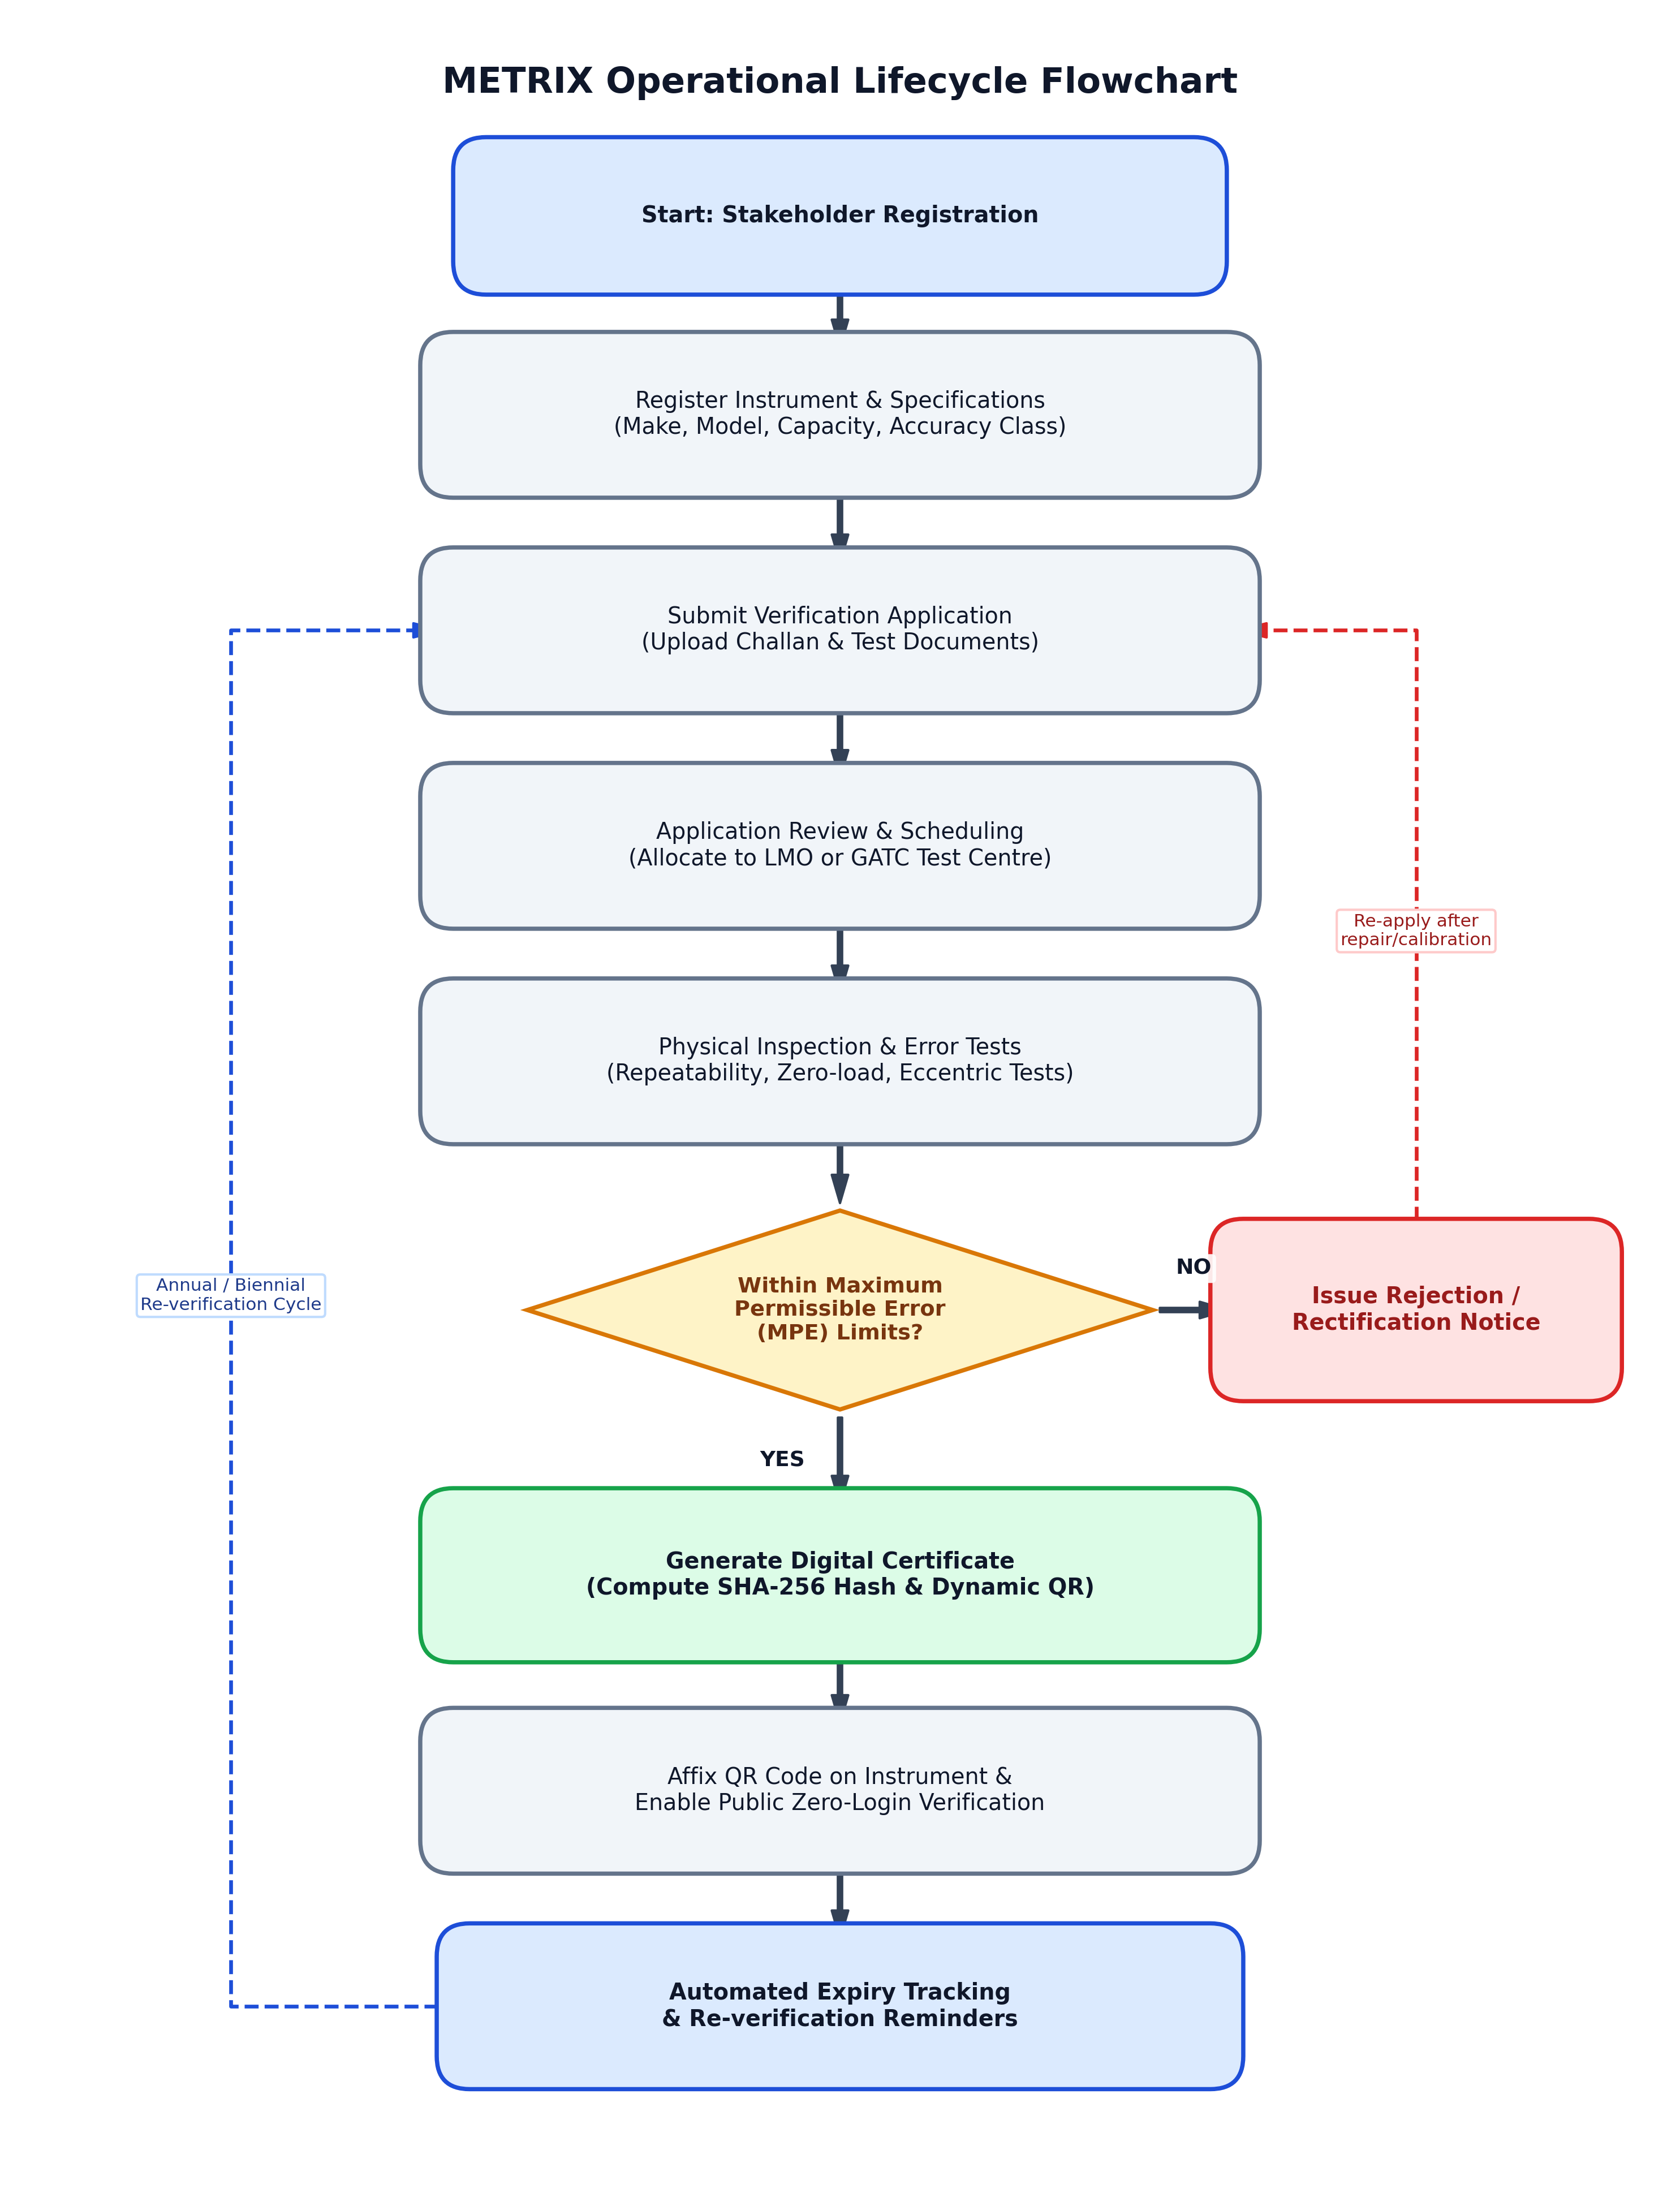
\includegraphics[width=0.82\textwidth]{process_flowchart.png}
\caption{Operational Lifecycle Flowchart of METRIX}
\label{fig:process_flowchart}
\end{figure}
